\documentclass[11pt]{article}
%-----------Packeges---------------%
\usepackage{amsmath}
\usepackage{amssymb}
\usepackage{amsfonts}
\usepackage{tocloft}
\usepackage{float}
\usepackage{graphicx}
\usepackage[bookmarks=true]{hyperref}
\usepackage{fancyhdr}


%----------Definition & Theorem----%
\newtheorem{definition}{Definition}[subsection]
\newtheorem{theorem}{Theorem}[subsection]
\newtheorem{proposition}{Proposition}[subsection]
\newtheorem{lemma}{Lemma}[subsection]
\newtheorem{corollary}{Corollary}[subsection]

\usepackage{tikz}
\begin{document}
	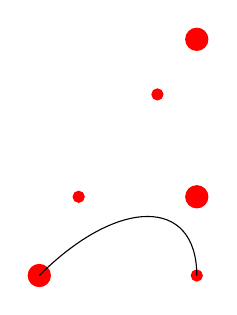
\begin{tikzpicture}
		\filldraw [red] 
			(0,0) circle [radius=4pt]
			(0.5,1) circle [radius=2pt] 
			(2,1) circle [radius=4pt]
			(2,3) circle [radius=4pt]
			(1.5,2.3) circle [radius=2pt] 
			(2,0) circle [radius=2pt];
			\draw (0,0) .. controls (1,1) and (2,1) .. (2,0);
	\end{tikzpicture}
	
	\begin{tikzpicture}
  		\draw (-1.5,0) -- (1.5,0);
  		\draw (0,-1.5) -- (0,1.5);
	\end{tikzpicture}
	
	 \tikz \draw (-1.5,0) -- (1.5,0) -- (0,-1.5) -- (0,1.5);	
	\begin{tikzpicture}
  \draw (-1.5,0) -- (1.5,0);
  \draw (0,-1.5) -- (0,1.5);
  \draw (-1,0) .. controls (-1,0.555) and (-0.555,1) .. (0,1)
               .. controls (0.555,1) and (1,0.555) .. (1,0);
\end{tikzpicture}
\end{document}
